\section{Model and Serving Details}
\label{app:models}

We serve the three open-weight agent
models~\citep{deepseekai2026flashcard,qwen2026fp8card,cyankiwi2026minimaxawq,lin2023awq} on our cluster with vLLM, each from
a per-model profile the launcher expands into one \texttt{vllm serve} command,
and a sweep is one batch job per model per tier that launches the server and
runs that tier's papers as processes on the same node. The agent's \texttt{run\_gpu}
calls hold their own Slurm allocation (Appendix~\ref{app:harness}), so agent
compute is metered apart from the serving GPUs. Muse Spark 1.2 is reached
through the Meta Model API.
Table~\ref{tab:models} lists the four configurations.

{\footnotesize
\setlength{\tabcolsep}{3pt}
\begin{longtable}{@{}>{\raggedright\arraybackslash}p{2.5cm}>{\raggedright\arraybackslash}p{3.05cm}>{\raggedright\arraybackslash}p{2.35cm}>{\raggedright\arraybackslash}p{2.15cm}>{\raggedright\arraybackslash}p{3.05cm}@{}}
\toprule
Setting & DeepSeek-V4-Flash & Qwen3.6-27B & MiniMax-M2.7 & Muse Spark 1.2 \\
\midrule
\endfirsthead
\multicolumn{5}{@{}l}{\footnotesize\itshape Table~\ref{tab:models}, continued.} \\[3pt]
\toprule
Setting & DeepSeek-V4-Flash & Qwen3.6-27B & MiniMax-M2.7 & Muse Spark 1.2 \\
\midrule
\endhead
\midrule
\endfoot
\bottomrule
\noalign{\vskip 6pt}
\caption{Served configuration of the four agent models, from the tier launch
scripts and the serve profiles.}
\label{tab:models} \\
\endlastfoot
Served checkpoint &
\texttt{deepseek-ai/\allowbreak{}DeepSeek-\allowbreak{}V4-\allowbreak{}Flash-\allowbreak{}0731} &
\texttt{Qwen/\allowbreak{}Qwen3.6-\allowbreak{}27B-\allowbreak{}FP8} &
\texttt{cyankiwi/\allowbreak{}MiniMax-\allowbreak{}M2.7-\allowbreak{}AWQ-\allowbreak{}4bit} &
\texttt{muse-\allowbreak{}spark-\allowbreak{}1.2-\allowbreak{}contributor} \\
Advertised name & same as checkpoint & same as checkpoint &
\texttt{MiniMaxAI/\allowbreak{}MiniMax-\allowbreak{}M2.7} & same as checkpoint \\
Precision & native INT8/FP8 & FP8 & 4-bit AWQ (W4A16) & vendor-served \\
KV cache dtype & \texttt{fp8} & \texttt{fp8} & not set & vendor-served \\
GPUs per replica & 2 & 1 & 2 & vendor-served \\
Tensor parallel & 2 & 1 & 2 & vendor-served \\
Served context & 409{,}600 & 262{,}144 & 196{,}608 & 1{,}000{,}000 declared \\
Agent input ceiling & 376{,}832 & 229{,}376 & 163{,}840 & 967{,}232 \\
Reasoning setting & \texttt{thinking} true,
\texttt{reasoning\_effort} \texttt{max} & checkpoint default &
checkpoint default & \texttt{reasoning\_effort} \texttt{xhigh} \\
Temperature & not set & not set & not set & not set \\
\texttt{top\_p} & 0.95 & not set & not set & not set \\
Tool-call parser & \texttt{deepseek\_v4} & \texttt{qwen3\_coder} &
\texttt{minimax\_m2} & API \\
Reasoning parser & \texttt{deepseek\_v4} & \texttt{qwen3} &
\texttt{minimax\_m2} & API \\
\texttt{max\_num\_seqs} & not set & 32 & not set & vendor-served \\
Tool rounds & 300 & 300 & 300 & 300 \\
\end{longtable}
}

We produce the grades of record with a separate grading client on the
Anthropic Messages API with \texttt{claude-sonnet-5}, one agent loop over one
run bundle capped at 25 rounds, and re-grading a batch overwrites the verdict
stored on each run's record, so a re-graded sweep has one grader. We price GPU time at the \$2
per \mbox{H100-hour} of Section~\ref{subsec:experimental-setup} and grader tokens at
\$2 and \$10 per million input and output tokens~\citep{anthropic2026pricing}.

\paragraph{Token usage and cost.} We take token pricing from OpenRouter's
listing of each model provider's own endpoint, and Table~\ref{tab:cost} lists
the totals. For the three
cluster-served models we take the tokens produced on our cluster and price them
at that listed rate. Figure~\ref{fig:app-b-tokens} shows the tokens of
each labeled run by agent, Figure~\ref{fig:app-b-cost} its cost, and
Figure~\ref{fig:app-b-split} the split between tokens and GPU time.

\begin{figure}[ht]
\centering
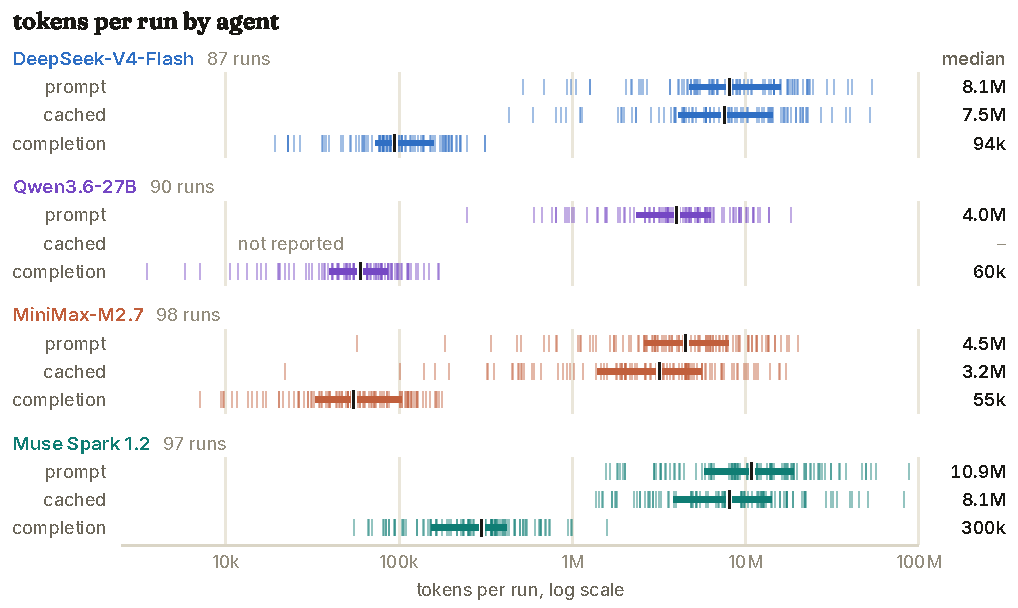
\includegraphics[width=\textwidth]{figures/app_B_tokens}
\caption{Prompt, cached prompt, and completion tokens per labeled run by agent on a shared log axis, one tick per run, with a bar over the middle half of runs and the median in black.}
\label{fig:app-b-tokens}
\end{figure}

\begin{figure}[ht]
\centering
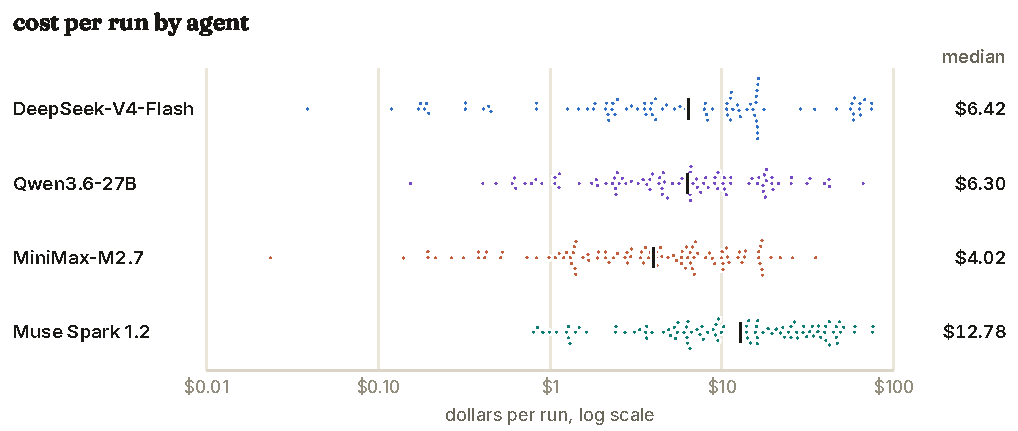
\includegraphics[width=\textwidth]{figures/app_B_cost}
\caption{Cost per labeled run by agent at the rates of Table~\ref{tab:cost}, with the median ticked.}
\label{fig:app-b-cost}
\end{figure}

\begin{figure}[ht]
\centering
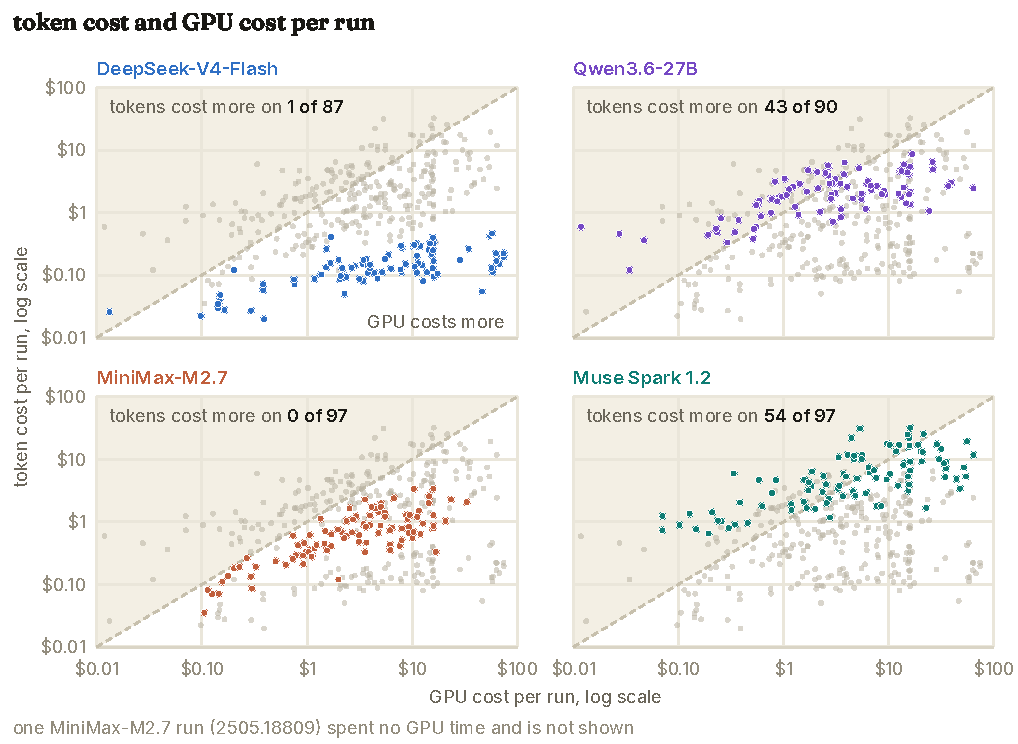
\includegraphics[width=\textwidth]{figures/app_B_split}
\caption{Token cost against GPU cost per labeled run by agent. The dashed line marks equal cost.}
\label{fig:app-b-split}
\end{figure}

\begin{table}[ht]
\centering
\fontsize{7.5}{9}\selectfont
\setlength{\tabcolsep}{0pt}
% wider gaps at the Rate | Tokens | Cost | Per run boundaries; the table fills the text width
\begin{tabular}{@{}l@{\hspace{9pt}}r@{\hspace{4.5pt}}r@{\hspace{4.5pt}}r@{\hspace{9pt}}r@{\hspace{4.5pt}}r@{\hspace{9pt}}r@{\hspace{4.5pt}}r@{\hspace{4.5pt}}r@{\hspace{9pt}}r@{}}
\toprule
& \multicolumn{3}{c}{Rate (\$/M)} & \multicolumn{2}{c}{Tokens (M)} &
\multicolumn{3}{c}{Cost (\$)} & \\
\cmidrule(lr){2-4} \cmidrule(lr){5-6} \cmidrule(lr){7-9}
Agent & Prompt & Cached & Completion & Prompt & Completion & Tokens & GPU &
Total & Per run \\
\midrule
DeepSeek-V4-Flash & 0.14 & 0.0028 & 0.28 & 1{,}077.9 & 11.11 & 15.04 & 1{,}337.64 & 1{,}352.68 & 13.66 \\
Qwen3.6-27B & 0.45 & -- & 2.70 & 489.1 & 6.24 & 236.93 & 797.63 & 1{,}034.56 & 10.45 \\
MiniMax-M2.7 & 0.30 & 0.06 & 1.20 & 573.8 & 6.62 & 82.21 & 528.61 & 610.82 & 6.17 \\
Muse Spark 1.2 & 1.25 & 0.15 & 4.25 & 1{,}494.6 & 33.53 & 724.91 & 1{,}112.34 & 1{,}837.24 & 18.56 \\
\midrule
All agents & & & & 3{,}635.4 & 57.50 & 1{,}059.08 & 3{,}776.22 & 4{,}835.30 & 12.21 \\
\bottomrule
\end{tabular}
\caption{Token usage and cost of the 396 runs that started.}
\label{tab:cost}
\end{table}

% No \FloatBarrier here: its \clearpage pushed B.1 onto a fresh page, leaving the rest of that page blank.
\subsection{Results by agent, tier, and compute band}
\label{app:results-table}

Table~\ref{tab:results} lists the values behind Figures~\ref{fig:main-results}
and~\ref{fig:band-compute}, where Reproduced counts a cell whose audit score is
8 or higher, a cell without a graded run counts as a failure at score 0, mean scores use the grades on the frozen targets,
grant spent is H100-hours used over hours
granted, and the band is the paper's H100-hour grant.

{\footnotesize
\setlength{\tabcolsep}{4pt}
\begin{longtable}{@{}llrrrrr@{}}
\toprule
& & \multicolumn{2}{c}{By tier} & \multicolumn{3}{c}{By band} \\
\cmidrule(lr){3-4} \cmidrule(l){5-7}
Agent & Tier or measure & Reproduced (95\% interval) & Mean score & 8 h & 32 h & 96 h \\
\midrule
\endfirsthead
\multicolumn{7}{@{}l}{\footnotesize\itshape Table~\ref{tab:results}, continued.} \\[3pt]
\toprule
& & \multicolumn{2}{c}{By tier} & \multicolumn{3}{c}{By band} \\
\cmidrule(lr){3-4} \cmidrule(l){5-7}
Agent & Tier or measure & Reproduced (95\% interval) & Mean score & 8 h & 32 h & 96 h \\
\midrule
\endhead
\endfoot
\bottomrule
\noalign{\vskip 6pt}
\caption{Reproduced cells, mean audit score, and grant spent over all 400
agent-paper cells, by agent, tier, and compute band.}
\label{tab:results} \\
\endlastfoot
DeepSeek-V4-Flash & Run & 13/34 (38\%, 24--55) & 5.29 (4.13--6.46) & & & \\*
& Retrain & 9/33 (27\%, 15--44) & 5.45 (4.40--6.51) & & & \\*
& Reimplement & 4/33 (12\%, 5--27) & 4.64 (3.79--5.49) & & & \\*
& All tiers & 26/100 (26\%, 18--35) & 5.13 (4.55--5.71) & & & \\*
& Mean score & & & 6.00 & 4.10 & 3.33 \\*
& Grant spent (\%) & \multicolumn{2}{r}{26.2 overall} & 42.0 & 34.0 & 13.5 \\
\midrule
Qwen3.6-27B & Run & 5/34 (15\%, 6--30) & 3.91 (2.97--4.85) & & & \\*
& Retrain & 6/33 (18\%, 9--34) & 3.58 (2.54--4.61) & & & \\*
& Reimplement & 2/33 (6\%, 2--20) & 3.03 (2.17--3.89) & & & \\*
& All tiers & 13/100 (13\%, 8--21) & 3.51 (2.98--4.04) & & & \\*
& Mean score & & & 4.03 & 3.14 & 1.83 \\*
& Grant spent (\%) & \multicolumn{2}{r}{15.6 overall} & 31.0 & 23.4 & 3.1 \\
\midrule
MiniMax-M2.7 & Run & 2/34 (6\%, 2--19) & 3.09 (2.09--4.09) & & & \\*
& Retrain & 5/33 (15\%, 7--31) & 3.30 (2.24--4.36) & & & \\*
& Reimplement & 1/33 (3\%, 1--15) & 2.70 (1.80--3.59) & & & \\*
& All tiers & 8/100 (8\%, 4--15) & 3.03 (2.48--3.58) & & & \\*
& Mean score & & & 3.56 & 2.41 & 1.92 \\*
& Grant spent (\%) & \multicolumn{2}{r}{10.4 overall} & 26.8 & 12.0 & 2.3 \\
\midrule
Muse Spark 1.2 & Run & 10/34 (29\%, 17--46) & 5.71 (4.81--6.60) & & & \\*
& Retrain & 8/33 (24\%, 13--41) & 5.85 (4.94--6.76) & & & \\*
& Reimplement & 5/33 (15\%, 7--31) & 3.85 (2.86--4.84) & & & \\*
& All tiers & 23/100 (23\%, 16--32) & 5.14 (4.59--5.69) & & & \\*
& Mean score & & & 5.85 & 4.55 & 3.08 \\*
& Grant spent (\%) & \multicolumn{2}{r}{21.8 overall} & 38.9 & 32.6 & 6.1 \\
\midrule
All agents & Run & 30/136 (22\%, 16--30) & 4.50 (3.98--5.02) & & & \\*
& Retrain & 28/132 (21\%, 15--29) & 4.55 (4.02--5.07) & & & \\*
& Reimplement & 12/132 (9\%, 5--15) & 3.55 (3.10--4.00) & & & \\*
& All tiers & 70/400 (18\%, 14--22) & 4.20 (3.91--4.49) & & & \\*
& Mean score & & & 4.86 & 3.55 & 2.54 \\*
& Grant spent (\%) & \multicolumn{2}{r}{18.5 overall} & 34.7 & 25.5 & 6.2 \\
\midrule
At least one agent & Run & 16/34 (47\%, 31--63) & & & & \\*
& Retrain & 11/33 (33\%, 20--50) & & & & \\*
& Reimplement & 5/33 (15\%, 7--31) & & & & \\*
& All tiers & 32/100 (32\%, 24--42) & & & & \\
% src: results/tiers/tier_tests.md (rebuttal/scripts/tier_tests.py), means and the at-least-one-agent rows
\end{longtable}
}

\subsection{Cells with no graded run, downloaded checkpoints, and failures outside the agent}
\label{app:outside-agent}

Of the 400 cells, 28 produced no graded run, and we traced each one through
the cluster's job accounting and the harness logs. Six failed outside the
agent, since the four cells of 2510.20725 never started because of a
prompt-rendering bug in our harness and two audits of Muse Spark 1.2 never
returned a verdict. Four of the other 22 were finished runs the pinned
auditor had not graded, and it has
now graded the three whose files survive at 0, 2, and 0, none of them
reproduced, while the fourth lost its files and stays ungraded. The pinned
auditor has also graded the two missing audits, reproduced (score 8) on
2503.23035 and partial (score 6) on 2510.08177. \todo{We reran the 4 cells of
2510.20725 with the same settings, and r of them reproduce.} Every rate in Section~\ref{subsec:results} and Table~\ref{tab:results} includes these grades, and a cell that
still has no graded run counts as a failure at score 0.
% src: replies.md:286-290; results/e8/summary.json (empty_cells: total 28; outside_agent_cells: 6); results/e8/d_cells.md and e8/regrade_dcells.json (3 of 4 regraded at 0, 2, 0; 2510.19314 ungraded); results/e8/README.md:19-27 (22 cells outside the first six, D 4); results/e8/regrade_muse.json (2503.23035 score 8, 2510.08177 score 6)

The harness keeps no network log, so we scanned every transcript, including
the commands, the fetched URLs, and the code the agent wrote, for downloads of
model weights. The scan finished on 368 of the 372 graded runs, none of the
four it could not finish was reproduced, and it covered all 42 reproduced
Retrain and Reimplement runs. Of the 16 of these with a match, two evaluated a
downloaded checkpoint of the model the claim is about, Muse Spark 1.2 on
2508.21046 at Retrain and MiniMax-M2.7 on 2505.12677 at Reimplement. Because
these tiers ask the agent to train or rebuild that model, we count both runs
as not reproduced, which lowers Muse Spark 1.2 to 8 of 33 at Retrain and
MiniMax-M2.7 to 1 of 33 at Reimplement, and the best Reimplement rate stays 5 of 33. The scan does not detect a download made inside an imported library.
% src: results/e9/README.md:12-19 (368/372 scanned; 4 timeouts; Retrain 13 of 29 and Reimplement 3 of 13 reproduced runs with a hit, 16 in all; class c 2); results/e9/class_review.csv rows 20-24; results/e8/bound.csv (muse retrain 9/33, minimax reimplement 2/33 before the correction)

Removing the 24 Build and dependency runs from the denominators
(Section~\ref{subsec:mechanisms}) leaves DeepSeek-V4-Flash at 13 of 34 at Run
and 9 of 33 at Retrain (27\%, 15\% to 44\%), since it has none of them at
either tier. Muse Spark 1.2, the best agent at Reimplement, goes from 5 of 33
(15\%, 7\% to 31\%) to 5 of 32 (16\%, 7\% to 32\%), and MiniMax-M2.7 at Run,
the agent most affected, goes from 2 of 34 to 2 of 26.% src: results/e8/bound.csv; results/e8/summary.json; results/e7/rescore_summary.md

For the re-execution of Section~\ref{subsec:mechanisms}, we took runs labeled Ran, outside tolerance at the Run and Retrain tiers in the 0--8 H100-hour band, and only three had a single command chain that ran without code the agent had edited by hand or several GPU sessions.

\subsection{Frontier models and production harnesses}
\label{app:frontier}

The frontier arms use the 12 core papers of a sample drawn with seed 22528,
four per tier, two of which some main agent had reproduced and two of which
none had, and the 12 extension papers drawn the same way. We froze the
sample before any frontier run and excluded 2510.20725, whose main-roster
cells never started. Each run gets the paper's band ceiling as its GPU grant,
the task text of the main runs, the same sandbox and \texttt{run\_gpu} tool, and
the pinned auditor. In Codex CLI and mini-SWE-agent the agent keeps the
harness's own tools, system prompt, and context handling, and a run ends when
the agent ends its own turn, which is the stopping rule of our harness.
Table~\ref{tab:frontier} gives the results beside DeepSeek-V4-Flash and Muse
Spark 1.2 on the same papers, and Muse Spark 1.2 against Muse Wonder compares
two models from one family. % src: results/subset/README.md (counts per tier and band; 2510.20725 excluded)

\begin{table}[ht]
\centering
\small
{\footnotesize\setlength{\tabcolsep}{4pt}% generated by rebuttal/scripts/frontier_tex.py; do not edit
\begin{tabular}{@{}llrlrrr@{}}
\toprule
& & & & & \multicolumn{2}{c}{Reproduced on the same papers} \\
\cmidrule(l){6-7}
Model & Harness & Papers & \shortstack{Reproduced\\(95\% interval)} & \shortstack{Mean\\score} & \shortstack{DeepSeek-\\V4-Flash} & \shortstack{Muse Spark\\1.2} \\
\midrule
gpt-6.1-sol & ours & 12 & 5 (19--68\%) & 5.67 & 4 & 4 \\
gpt-6.1-sol & Codex CLI & 23 & 4 (7--37\%) & 5.00 & 8 & 7 \\
gpt-6.1-sol & Codex CLI + prompts & 3 & 2 (21--94\%) & 7.67 & 3 & 1 \\
gpt-6-astra & ours & 6 & 1 (3--56\%) & 4.83 & 4 & 3 \\
gpt-6-astra & Codex CLI & 8 & 2 (7--59\%) & 4.38 & 4 & 3 \\
Muse Wonder & ours & 1 & 0 (0--79\%) & 3.00 & 0 & 0 \\
Muse Wonder & mini-SWE-agent & 6 & 4 (30--90\%) & 6.83 & 3 & 2 \\
\bottomrule
\end{tabular}
}
\caption{Papers reproduced by each frontier arm, beside the two best open
agents on the papers that arm has graded.}
\label{tab:frontier}
\end{table}
% src: results/databook/frontier_cells.csv through rebuttal/scripts/frontier_tex.py; moves with: the remaining frontier runs
\todo{Tables~\ref{tab:frontier} and~\ref{tab:frontier-runs} hold the runs
graded by 11-09 and are regenerated before upload.}

The open-agent columns use the submitted grade of that agent on the same
papers. Because half of the sampled papers are ones some open agent had
reproduced under the submitted grades, those columns favor the open agents, so we also reran
DeepSeek-V4-Flash twice on the 12 core papers, where it reproduces \todo{r2}
and \todo{r3}. \todo{With up to three prompts to continue after the agent ends
its turn, gpt-6.1-sol in Codex CLI reproduces f of 8 papers.} The frontier runs
spend a median of \todo{2.1}\% of their GPU grant, against \todo{17.2}\% for
the open agents on the same papers, and Table~\ref{tab:frontier-runs} lists
every run with its exit reason. We did not run Claude Code, since the auditor
is a Claude model. Under the submitted grades some agent reproduced 34 of the 99 papers the sample was drawn from, so the sample holds a larger share of reproduced papers than the benchmark.
% src: results/frontier/same_paper_baselines.md; repeat runs jobs 3540624 to 3540633; continue-prompt variant: results/databook/frontier_cells.csv arm codex-gpt-6.1-sol-nudge when graded

% generated by rebuttal/scripts/frontier_tex.py; do not edit
{\scriptsize
\setlength{\tabcolsep}{3pt}
\begin{longtable}{@{}lllllrl@{}}
\toprule
Model & Harness & Paper & Tier & Verdict (score) & Grant spent (\%) & Exit reason \\
\midrule
\endhead
\endfoot
\bottomrule
\noalign{\vskip 6pt}
\caption{Every graded frontier run with its verdict, the share of its GPU
grant it spent, and its exit reason.}
\label{tab:frontier-runs} \\
\endlastfoot
gpt-6.1-sol & ours & 2502.05795 & Run & reproduced (8) & 83.7 & agent ended the run \\
gpt-6.1-sol & ours & 2503.02809 & Reimplement & reproduced (8) & 1.5 & agent ended the run \\
gpt-6.1-sol & ours & 2503.14698 & Reimplement & unverifiable (1) & 0.0 & agent ended the run \\
gpt-6.1-sol & ours & 2504.12463 & Retrain & not reproduced (2) & 0.3 & agent ended the run \\
gpt-6.1-sol & ours & 2504.20571 & Run & reproduced (8) & 15.7 & agent ended the run \\
gpt-6.1-sol & ours & 2505.16927 & Reimplement & unverifiable (1) & 0.2 & agent ended the run \\
gpt-6.1-sol & ours & 2505.19087 & Reimplement & partial (7) & 3.3 & agent ended the run \\
gpt-6.1-sol & ours & 2506.06991 & Retrain & partial (6) & 13.8 & agent ended the run \\
gpt-6.1-sol & ours & 2506.08898 & Retrain & not reproduced (4) & 0.6 & agent ended the run \\
gpt-6.1-sol & ours & 2506.20671 & Run & reproduced (8) & 13.8 & agent ended the run \\
gpt-6.1-sol & ours & 2510.21363 & Retrain & partial (7) & 87.0 & agent ended the run \\
gpt-6.1-sol & Codex CLI & 2412.11979 & Run & not reproduced (2) & 1.2 & agent ended the run \\
gpt-6.1-sol & Codex CLI & 2503.02809 & Reimplement & partial (7) & 0.7 & agent ended the run \\
gpt-6.1-sol & Codex CLI & 2503.14698 & Reimplement & not reproduced (2) & 0.0 & agent ended the run \\
gpt-6.1-sol & Codex CLI & 2504.12463 & Retrain & not reproduced (2) & 0.2 & agent ended the run \\
gpt-6.1-sol & Codex CLI & 2504.20571 & Run & reproduced (8) & 10.6 & GPU grant spent \\
gpt-6.1-sol & Codex CLI & 2505.12677 & Reimplement & partial (6) & 3.2 & agent ended the run \\
gpt-6.1-sol & Codex CLI & 2505.16927 & Reimplement & unverifiable (1) & 0.2 & agent ended the run \\
gpt-6.1-sol & Codex CLI & 2505.18809 & Run & not reproduced (4) & 13.6 & agent ended the run \\
gpt-6.1-sol & Codex CLI & 2505.19087 & Reimplement & reproduced (8) & 2.1 & agent ended the run \\
gpt-6.1-sol & Codex CLI & 2505.19154 & Run & partial (6) & 7.2 & agent ended the run \\
gpt-6.1-sol & Codex CLI & 2506.08898 & Retrain & not reproduced (4) & 1.9 & agent ended the run \\
gpt-6.1-sol & Codex CLI & 2506.20671 & Run & not reproduced (2) & 2.1 & agent ended the run \\
gpt-6.1-sol & Codex CLI & 2510.21363 & Retrain & partial (7) & 52.8 & agent ended the run \\
gpt-6.1-sol & Codex CLI & 2511.01463 & Reimplement & not reproduced (2) & 0.2 & agent ended the run \\
gpt-6.1-sol & Codex CLI & 2602.03066 & Reimplement & partial (7) & 1.5 & agent ended the run \\
gpt-6-astra & ours & 2504.20571 & Run & reproduced (8) & 0.0 & agent ended the run \\
gpt-6-astra & ours & 2505.16927 & Reimplement & unverifiable (1) & 0.0 & agent ended the run \\
gpt-6-astra & ours & 2506.08898 & Retrain & not reproduced (4) & 0.0 & agent ended the run \\
gpt-6-astra & Codex CLI & 2504.12463 & Retrain & not reproduced (2) & 0.2 & agent ended the run \\
gpt-6-astra & Codex CLI & 2504.20571 & Run & not reproduced (2) & 5.1 & time limit \\
gpt-6-astra & Codex CLI & 2505.10475 & Run & not reproduced (3) & 2.9 & time limit \\
gpt-6-astra & Codex CLI & 2505.16927 & Reimplement & unverifiable (1) & 0.1 & agent ended the run \\
gpt-6-astra & Codex CLI & 2505.19087 & Reimplement & reproduced (8) & 2.6 & agent ended the run \\
gpt-6-astra & Codex CLI & 2506.08898 & Retrain & not reproduced (2) & 0.5 & agent ended the run \\
gpt-6-astra & Codex CLI & 2510.21363 & Retrain & not reproduced (4) & 4.9 & agent ended the run \\
Muse Wonder & mini-SWE-agent & 2505.10475 & Run & reproduced (8) & 41.5 & agent ended the run \\
Muse Wonder & mini-SWE-agent & 2505.16927 & Reimplement & not reproduced (3) & 5.6 & agent ended the run \\
Muse Wonder & mini-SWE-agent & 2506.08898 & Retrain & partial (6) & 0.9 & agent ended the run \\
\end{longtable}
}


\FloatBarrier  % no Appendix C float prints above the continued part of Table 5
